\documentclass[a4paper,10pt]{article}

% ---------------- PACCHETTI ----------------
\usepackage[utf8]{inputenc}       % encoding
\usepackage[T1]{fontenc}          % font encoding
\usepackage[italian]{babel}       % lingua italiana
\usepackage{graphicx}             % immagini
\usepackage{amsmath, amssymb}     % matematica
\usepackage{listings}             % codice sorgente
\usepackage{xcolor}               % colori
\usepackage{hyperref}             % link cliccabili
\usepackage{geometry}             % margini pagina
\usepackage{mdframed}
\usepackage{booktabs}
\usepackage{subcaption}
\usepackage{hyperref}
\geometry{margin=2.5cm}

\newmdenv[linecolor=black,linewidth=0.5pt,backgroundcolor=gray!10]{defbox}
\newmdenv[linecolor=black,linewidth=0.5pt,backgroundcolor=white!10]{citabox}

\newcommand{\mousedx}{
\includegraphics[scale=0.6]{Assets/mousedx.pdf}}
\newcommand{\mousesx}{
\includegraphics[scale=0.6]{Assets/mousesx.pdf}}

% ---------------- STILE CODICE ----------------
\lstset{
	language=C++,
	basicstyle=\ttfamily\small,
	keywordstyle=\color{blue},
	stringstyle=\color{orange},
	commentstyle=\color{gray},
	numbers=left,
	numberstyle=\tiny,
	stepnumber=1,
	numbersep=5pt,
	frame=single,
	breaklines=true
}

% ---------------- DOCUMENTO ----------------
\begin{document}
	
	\begin{titlepage}
		\centering
		\vspace*{\fill}
		{\huge \textbf{Progetto in C++, framework Qt}}\\[0.5cm]
		{\Huge \textbf{MyDigitalLibrary}}\\[1.5cm]
		
		\rule{\textwidth}{0.5pt}\\[0.4cm] % linea orizzontale elegante
		{\LARGE Relazione tecnica}\\[0.1cm]
		\rule{\textwidth}{0.5pt}\\[2cm]
		
		\begin{flushright}
		{\Large \textbf{Università degli Studi di Padova}} \\[0.1cm]
		{\Large \textbf{L.T. in Informatica}} \\[0.1cm]
		{\Large \textbf{A.A. 2024/25}} \\[0.5cm]
		\end{flushright}
		
		\begin{flushleft}
			\textbf{Autore} Thomas Morettin \\
			\textbf{\hspace*{0.5cm}Matr.} 2111001 \\[0.5cm]
			\textbf{Data} 07.09.2025 \\
			\textbf{Corso} Programmazione ad Oggetti \\
			\textbf{\hspace*{0.5cm}Cod.} SC02123180 \\
		\end{flushleft}
		\vspace*{\fill}
	\end{titlepage}
	\tableofcontents
	\clearpage
	
	\section{Introduzione}
	\textbf{MyDigitalLibrary} è un prodotto software che opera come \textit{libreria digitale}. Esso permette la memorizzazione e la gestione di diverse tipologie di \textbf{Media}, i quali si dividono in: \textbf{Album, Film, Libri e Riviste}.\\ Le funzionalità principali che offre riguardano la memorizzazione dei Media, i quali vengono visualizzati all'interno di un catalogo che offre una vista su tutti o alcuni elementi filtrati grazie a criteri di ricerca, e la loro gestione; nello specifico si fa riferimento ad operazioni che permettono:
	\begin{itemize}
		\item inserimento di nuovi Media;
		\item visualizzazione in dettaglio del Media;
		\item eliminazione del Media;
		\item modifica di tutti o alcuni dati del Media;
		\item import/export da file JSON.
	\end{itemize}
	Per concludere, l'applicazione è progettata con un'interfaccia grafica comprensibile e minimale, per offrire all'utente un'esperienza di utilizzo semplice e curata.
	
	\section{Descrizione del modello}\label{def:MVC}
	Di seguito viene riportato un estratto del \textbf{diagramma UML} delle classi dell'applicazione, reperibile nella sua forma integrale all'interno della cartella contenente la presente relazione tecnica, al nome di \texttt{DiagrammaUML.svg}.
	\begin{figure}[h!]
		\centering
		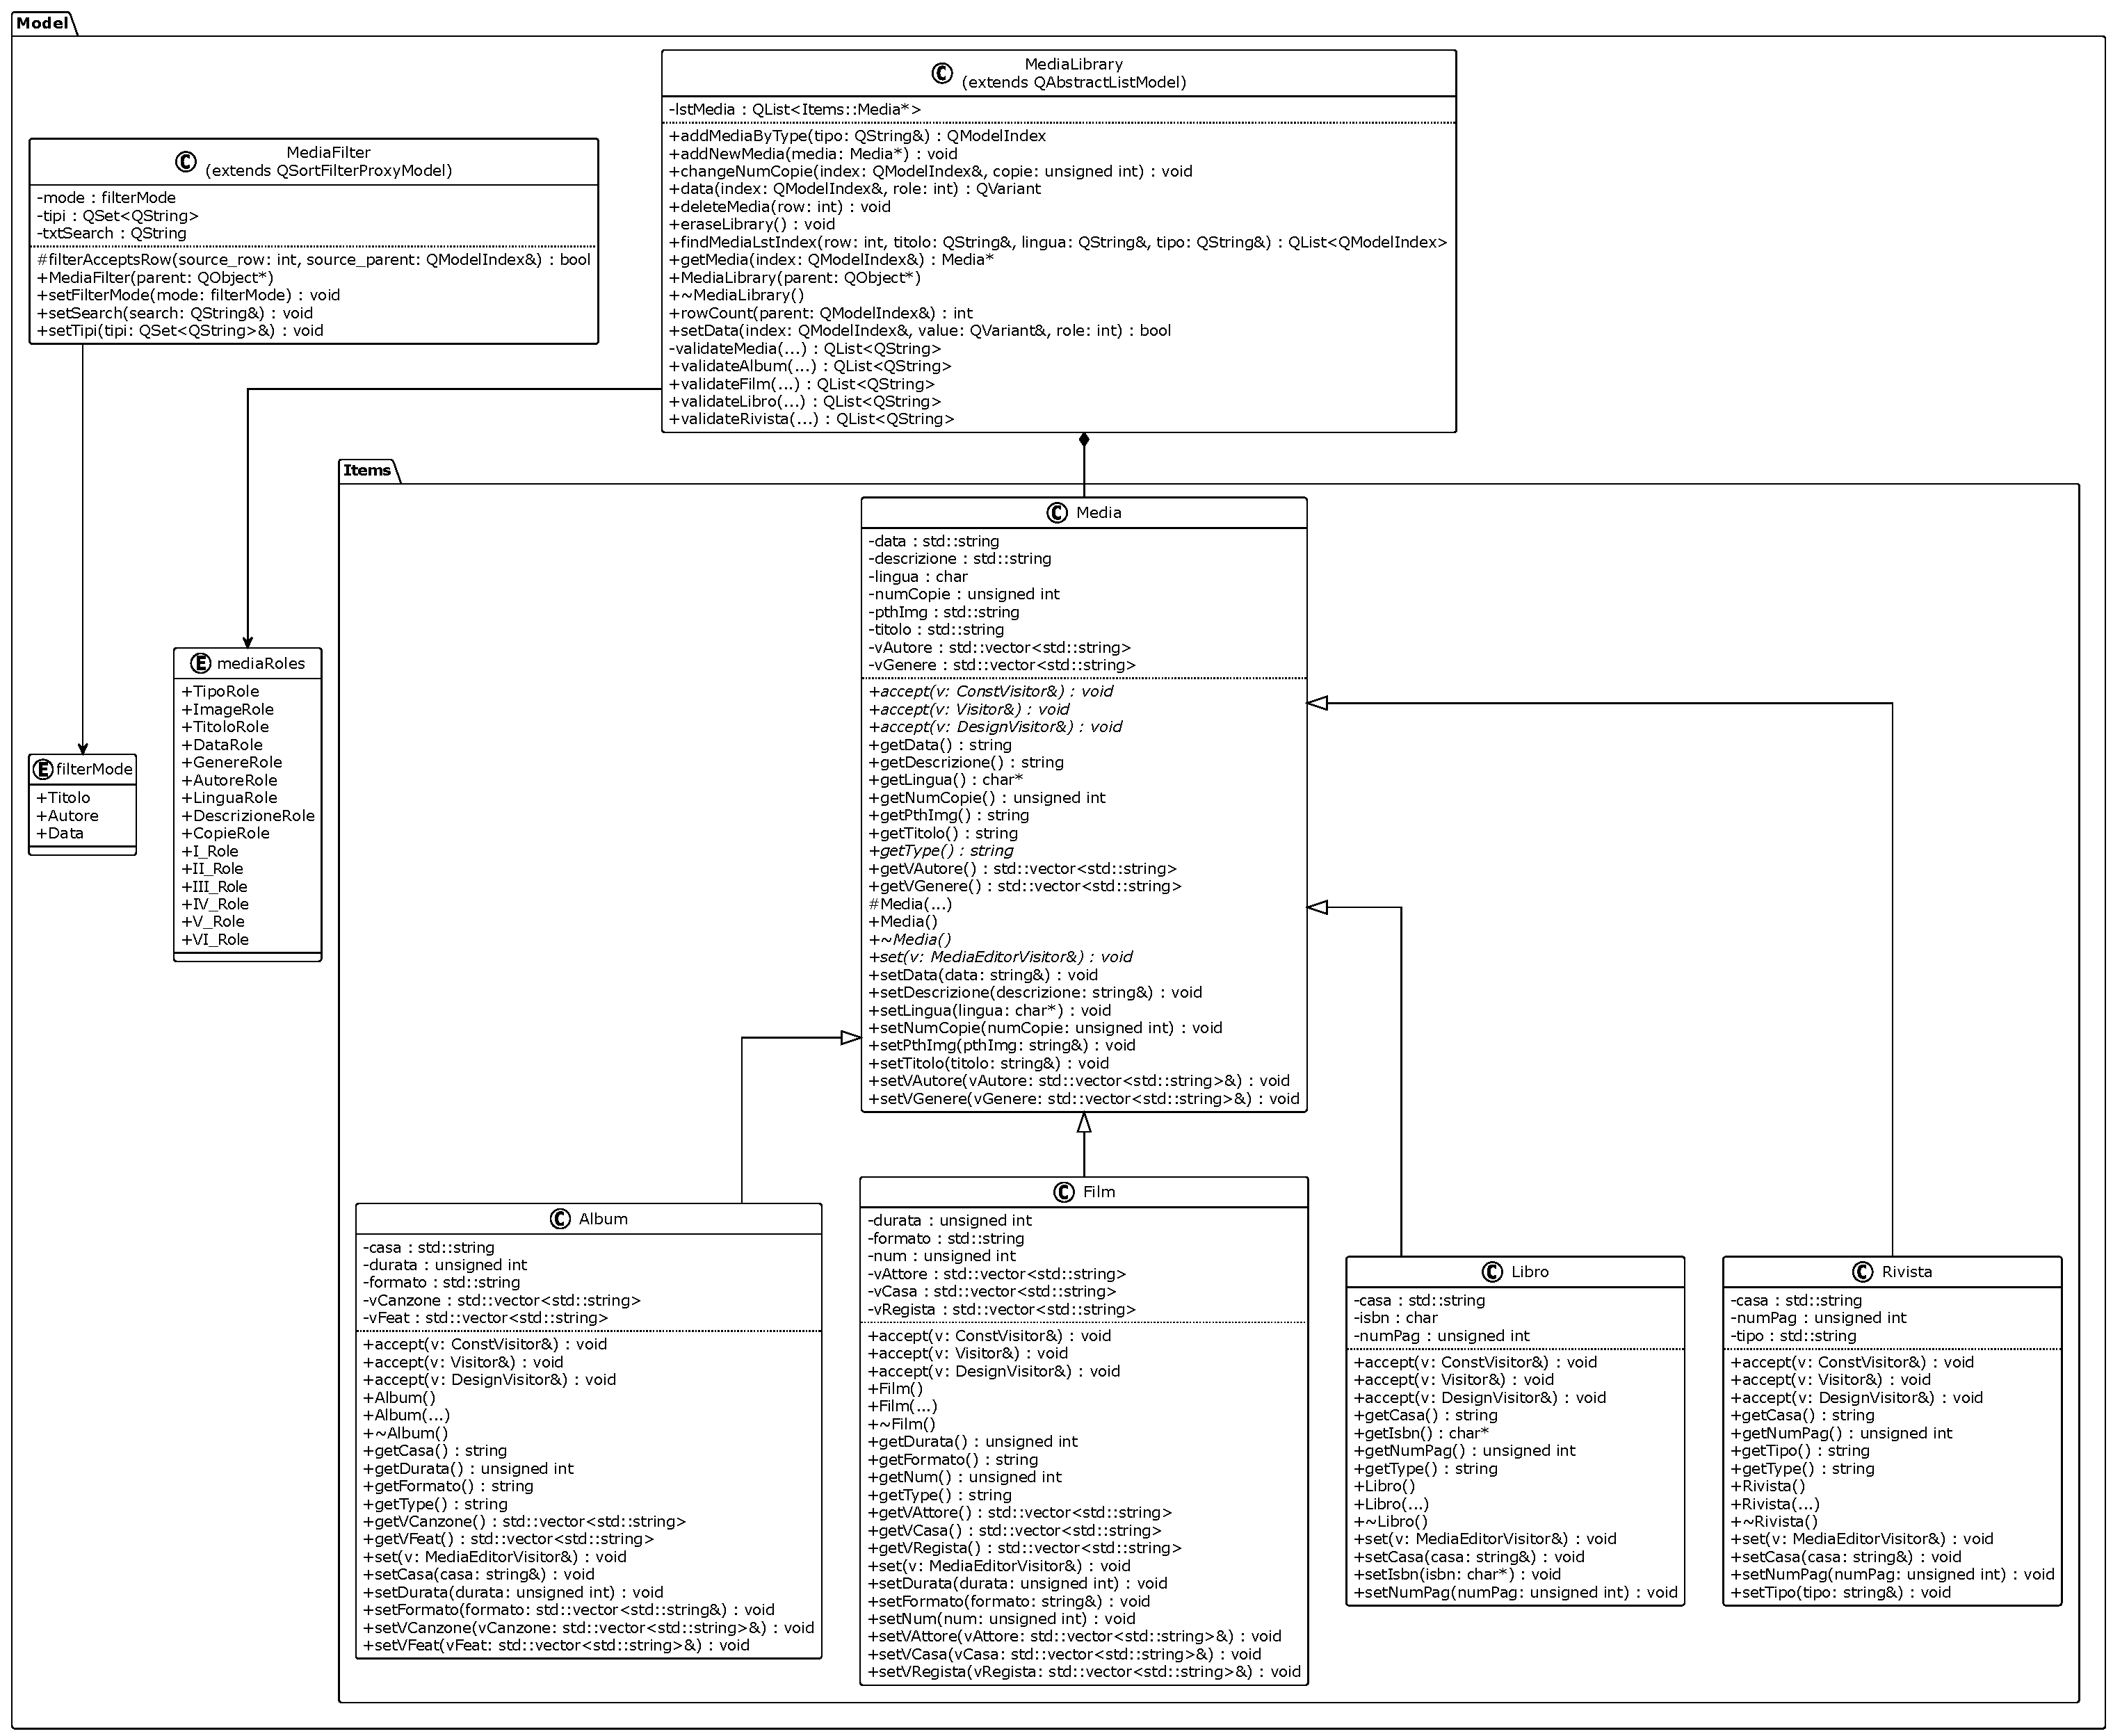
\includegraphics[scale=0.3]{Assets/diagrammaereditarieta.pdf}
		\caption{Diagramma UML delle classi fondamentali}
		\label{fig:diagramma}
	\end{figure}\\
	Per la realizzazione del prodotto si è fatto riferimento al \textbf{design pattern MVC}, ovvero lo scheletro principale dell'intera applicazione.
	\begin{defbox}
	\textbf{MVC}, acronimo di Model View Controller, è un design pattern architetturale che impone la separazione tra la logica di presentazione dei dati e la loro logica di business (manipolazione).\\
	La struttura è cosi composta:
	\begin{itemize}
		\item \textbf{Model} ha il compito di memorizzare i dati dell'applicazione;
		\item \textbf{View} rappresenta la visualizzazione grafica degli elementi;
		\item \textbf{Controller} è il gestore del \textit{Model}, pertanto ha il compito di notificare la \textit{View} dei cambiamenti del Model e manipolare quest'ultimo.
	\end{itemize}
	\end{defbox}
	Il progetto, seguendo le specifiche del design pattern MVC, è così organizzato:
	\begin{itemize}
		\item \textbf{\texttt{MediaLibrary}} è la classe con il ruolo di \textit{Controller}, pertanto al suo interno sono stati implementati tutti i metodi che permettono la manipolazione del \textit{Model}, il quale è rappresentato da una \texttt{QList<Items::Media*>} (privata) per la memorizzazione degli oggetti Media.\\
		La suddetta classe estende la classe \texttt{QAbstractListModel}, ovvero un'interfaccia standard, offerta dal framework Qt, per l'implementazione del design pattern MVC. Inoltre, presenta un campo \texttt{enum} adibito al riconoscimento dei ruoli di ciascun Media, ovvero i suoi dati sui quali possono essere implementate le operazioni CRUD.
		\item \textbf{\texttt{Media}} rappresenta la classe base astratta (con campi generici comuni a tutti gli oggetti concreti), da cui ereditano tutte le classi concrete che rappresentano gli oggetti manipolabili all'interno dell'applicazione con i propri campi specifici.\\
		\item \textbf{\texttt{MainWindow, FnsIniziale, FnsCatalogo, FnsDettagli e FrmEditor}} sono le classi che hanno il ruolo di \textit{View}, ovvero permettono la visualizzazione dei dati. Per semplicità le classi non sono state riportate nel Figura~\ref{fig:diagramma} a pag.~\pageref{fig:diagramma}, ma di seguito viene riportata la loro struttura:
		\begin{itemize}
			\item \textbf{\texttt{MainWindow}} rappresenta la finestra principale, la quale grazie ad un oggetto \texttt{QStackedWidget} permette di gestire dinamicamente le finestre per le operazioni all'utente;
			\item \textbf{\texttt{FnsIniziale}} rappresenta la finestra iniziale dalla quale è possibile istanziare la libreria. Successivamente all'instanza della libreria, prima di essere distrutta, viene inviato un segnale a tutte le finestre per la memorizzazione della libreria creata;
			\item \textbf{\texttt{FnsCatalogo}} rappresenta la finestra principale dove è possibile svolgere la maggior parte delle operazioni, inclusa la visualizzazione della \texttt{QListView} per la lista di Media. Il precedente oggetto è collegato alla classe \texttt{MediaFilter}, la quale estendendo \texttt{QSortFilterProxyModel} ha il compito di visualizzare gli elementi filtrati tramite i criteri di ricerca, prelevando i dati direttamente dal \textit{Model} dell'applicazione;
			\item \textbf{\texttt{FnsDettagli}} rappresenta la finestra di visualizzazione di tutti i dettagli di un oggetto Media, facendo uso del Visitor MediaDettagliVisitor (Sezione~\ref{def:visitor} a pag.~\pageref{def:visitor}, il quale si occupa della creazione dei campi generici e specifici (con il loro popolamento);
			\item \textbf{\texttt{FrmEditor}} rappresenta la finestra di modifica dei dati di un oggetto Media, facendo uso del Visitor \texttt{MediaEditorVisitor} (Sezione~\ref{def:visitor} a pag.~\pageref{def:visitor}, il quale si occupa della creazione dei campi di input generici e specifici (con il loro popolamento).\\
			\begin{quote}
				\textbf{NB} La suddetta classe viene utilizzata sia per l'inserimento di un nuovo Media che per la sua successiva modifica, questo per rendere lo sviluppo più efficiente e mantenibile nel tempo.\\
				Il segnale di annullamento dell'inserimento/modifiche aziona due slot differenti all'interno della \texttt{MainWindow}, per il corretto funzionamento del programma.
			\end{quote}
		\end{itemize}
	\end{itemize}
	Per l'applicazione, oltre al design pattern MVC, è stato fatto uso del \textbf{design pattern Visitor} per la corretta gestione degli oggetti concreti derivanti da Media (spiegato esaustivamente nella sezione successiva) e del \textbf{design pattern Factory}, il quale viene implementato nella classe \texttt{MediaFactory} per la creazione di un oggetto \texttt{QJsonObject} per ciascun Media, da poter inserire all'interno del file portabile JSON.
	
	\clearpage
	\section{Polimorfismo}
	Nella presente applicazione si è sfruttato il concetto di polimorfismo sia nella variante "banale" imposta dal linguaggio di programmazione C++, che "non banale" tramite l'utilizzo di \textbf{design pattern Visitor}.
	\begin{defbox}
		\textbf{Visitor} è un design pattern comportamentale, il quale ha il compito di separare un algoritmo dalla struttura dati alla quale è applicato. Ciò viene utilizzato per aggiungere nuove funzionalità senza dover modificare la struttura base degli oggetti sui quali è applicato.\\
		Il suo utilizzo risulta fondamentale, nel contesto di quest'applicazione, nella gestione di algoritmi differenti per tipo concreto dell'oggetto visitato.
	\end{defbox}
	\begin{quote}
		\textbf{NB} Tutte le classi che fanno uso di design pattern Visitor sono state create con lo scopo sia di gestire i campi generici di ciascun Media (\textbf{es} lingua, titolo, ...) che quelli specifici per tipologia (\textbf{es} Libro → ISBN, Album → durata, ...) per maggiore manutenibilità del codice.
	\end{quote}
	
	\subsection{Visitor::Items::MediaGetterVisitor/MediaSetterVisitor}
	Il primo utilizzo di polimorfismo "non banale" riguarda le classi che permettono di estrarre e settare i parametri, di ciascun Media. Le classi, rispettivamente figlie delle classi \texttt{ConstVisitor e Visitor}, permettono di manipolare i ruoli definiti all'interno del \textit{Model} che gestisce la \texttt{QList<Items::Media*>}.
	
	\subsection{Visitor::JSON::ToJsonVisitor}
	Il secondo utilizzo avviene nella classe adibita alla creazione di un oggetto \texttt{QJsonObject} a partire dal Media, per tipologia, presente nel catalogo, per il popolamento del file JSON.
	
	\subsection{Visitor::View::MediaDettagliVisitor/MediaEditorVisitor}\label{def:visitor}
	L'utilizzo più significativo di polimorfismo all'interno dell'applicazione avviene nelle suddette classi, le quali ereditano dalla classe base astratta \texttt{DesignVisitor}.\\
	La classe \texttt{MediaDettagliVisitor} fa uso di design pattern Visitor per la creazione e il popolamento dei widget \texttt{QLabel} adibiti alla visualizzazione dei dettagli generici e specifici (per tipologia) di ciascun Media.
	La classe \texttt{MediaEditorVisitor} si occupa della creazione, del popolamento e del controllo dei widget \texttt{QLineEdit, QTextEdit e QComboBox}, adibiti all'inserimento/modifica delle informazioni generiche e specifiche (per tipologia) di ciascun Media. Ulteriormente, la classe \texttt{MediaEditorVisitor} implementa metodi \texttt{set()}, non presenti nella classe base astratta, per effettuare il popolamento/modifica (dagli elementi widget) delle informazioni di ciascun Media tramite i ruoli del \textit{Model} mantenendo separate le responsabilità dettate dal design pattern MVC (Sezione~\ref{def:MVC} a pag.~\pageref{def:MVC}).\\
	Quest'ultima classe, inoltre, implementa metodi, propri per ciascuna tipologia di Media, per la chiamata a funzioni di validazione dei dati (interne alla classe \texttt{MediaLibrary}) forniti dall'utente (\textbf{es} il Libro presenta codice ISBN nel formato corretto), con conseguente avviso all'utente nel caso in cui tenti di salvare dati non coerenti con la struttura degli oggetti del prodotto software.\\
	\begin{quote}
		\textbf{NB} Entrambe le classi restituiscono un oggetto \texttt{QWidget}, contenente le informazioni generiche e specifiche per tipologia di Media.\\
		Inoltre, entrambe le classi \texttt{MediaDettagliVisitor} e \texttt{MediaEditorVisitor} sovrascrivono un metodo virtuale pure, definito nella classe base \texttt{DesignVisitor}, dal nome \texttt{clear()} che permette di distruggere il \texttt{QWidget} contenente i campi specifici per ciascun Media. In questo modo, nel caso in cui il Media selezionato dall'utente dovesse essere differente rispetto al precedente, la finestra viene aggiornata inserendo i campi di input corretti; se questo dovesse essere identico, invece, il visitor non procederà alla distruzione del \texttt{QWidget} per gli elementi specifici ma aggiornerà semplicemente i campi nel caso in cui siano stati aggiornati.
	\end{quote}
	
	\subsection{Visitor::Items::CheckFormatoVisitor}
	L'ultimo utilizzo di polimorfismo avviene nella classe che, ereditando da \texttt{ConstVisitor}, ha il compito di controllare l'uguaglianza tra un parametro fornito dalla ricerca ne \texttt{QList<Items::Media*>} e i seguenti campi per ciascun Media: \textbf{Album → formato, Film → formato, Libro → ISBN e Rivista → tipo}. Questa classe viene utilizzata per la gestione dei duplicati, insieme alla corrispondenza lingua/titolo (Sezione~\ref{sec:duplicati} a pag.~\pageref{sec:duplicati}).
	
	\clearpage
	\section{Persistenza dei dati}
	Come da commessa accademica è stato progettato un sistema di persistenza dei dati su file system tramite file in formato \textbf{JSON}. Nello specifico, il suddetto file contiene la memorizzazione dell'intero catalogo di oggetti Media, gestendone la specificità tramite un attributo \textit{media}.\\
	Viene consegnato, all'interno della cartella di progetto, un file \texttt{Savings/Salvataggio.json} (presente, identico, nella cartella \texttt{EsempioPersistenza} della \textbf{cartella ZIP} contenente l'intero lavoro), contenente diversi oggetti per tipologia, in modo da poter avviare il prodotto con Media pre registrati.
	\begin{quote}
		\textbf{NB} Il file JSON, oltre a contenere oggetti Media correttamente memorizzati, ne contiene alcuni che presentano dati mancanti, richiesti dalla struttura del codice per l'importazione. Ciò a dimostrazione di come alcuni Media potranno non essere importati correttamente, a causa delle \textbf{politiche di controllo} del file .json.\\
	\end{quote}
	
	\section{Funzionalità implementate}
	In aggiunta alle funzionalità richieste all'interno della commessa, vengono riportate di seguito le migliorie funzionali/grafiche implementate all'interno del prodotto software.
	\subsection{Implementazioni funzionali}
	\begin{figure}[h!]
		\centering
		\begin{subfigure}{0.3\textwidth}
			\centering
			
\includegraphics[scale=0.07]{Assets/btninformazioni.pdf}
			\caption{FnsIniziale}
			\label{fig:btninformazioni}
		\end{subfigure}
		\begin{subfigure}{0.3\textwidth}
			\centering
			
\includegraphics[scale=0.07]{Assets/btnerase.pdf}
			\caption{FnsCatalogo}
			\label{fig:btnerase}
		\end{subfigure}
		\begin{subfigure}{0.3\textwidth}
			\centering
			
\includegraphics[scale=0.07]{Assets/btnimportexport.pdf}
			\caption{FnsCatalogo}
			\label{fig:btnimportexport}
		\end{subfigure}\\[0.25cm]
		\begin{subfigure}{\textwidth}
			\centering
			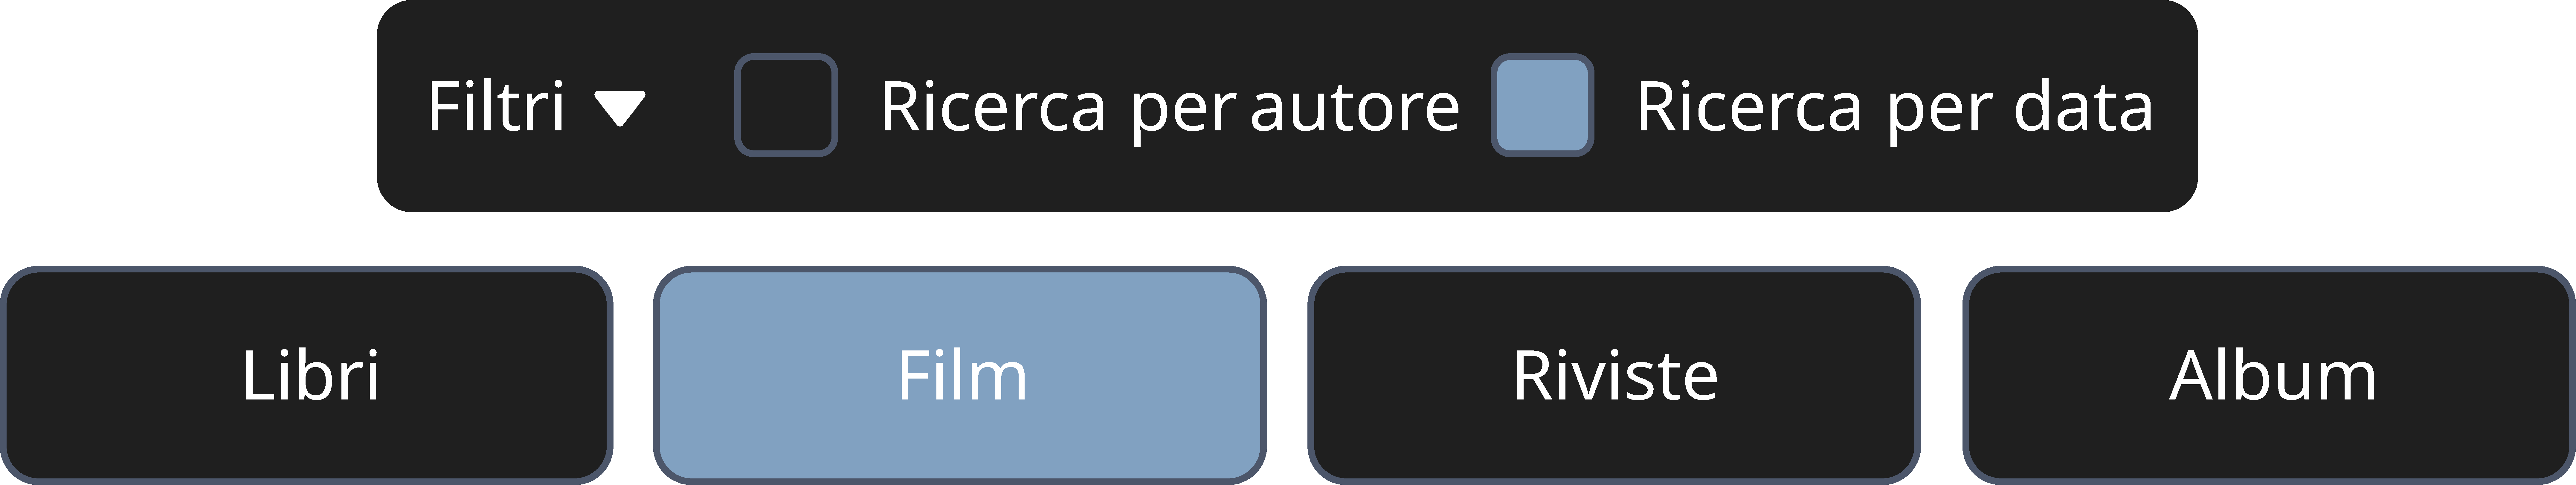
\includegraphics[scale=0.07]{Assets/filtri.pdf}
			\caption{FnsCatalogo}
			\label{fig:filtri}
		\end{subfigure}\\[0.25cm]
		\begin{subfigure}{0.4\textwidth}
			\centering
			
\includegraphics[scale=0.07]{Assets/lingue.pdf}
			\caption{FnsCatalogo/FnsDettagli/FrmEditor}
			\label{fig:lingue}
		\end{subfigure}
		\begin{subfigure}{0.4\textwidth}
			\centering
			
\includegraphics[scale=0.07]{Assets/btnrestore.pdf}
			\caption{FrmEditor}
			\label{fig:btnrestore}
		\end{subfigure}
		\caption{Elementi grafici in evidenza}
	\end{figure}
	Si considerino le seguenti:
	\begin{itemize}
		\item gestione di \textbf{quattro tipologie} di oggetti Media;
		\item importazione ed esportazione dei dati in formato JSON:
		\begin{itemize}
			\item controllo sulla \textbf{presenza e correttezza} dei campi dati memorizzati; nel caso di dati mancanti/incorretti espressamente richiesti a livello funzionale il Media non viene importato nella libreria, con avviso all'utente. Questo per mantenere il sistema robusto e permettere all'utente di poter inserire manualmente, nel file JSON, solamente i dati minimali, per completare il Media all'interno dell'applicazione.
			\begin{quote}
				\textbf{ES} Per tutti gli oggetti Libro è richiesto obbligatoriamente il campo ISBN in formato 13 char, altrimenti il Media non viene caricato.\\
				Per tutti gli oggetti Rivista viene controllata la presenza del campo casa editoriale, se questo dovesse essere errato o inesistente il Media viene importato correttamente nella libreria, ma alla prossima modifica ne è obbligatorio l'inserimento.
			\end{quote}
		\end{itemize}
		\item pulsante di apertura della documentazione tecnica dalla finestra di inizializzazione della libreria (path individuato automaticamente tramite variabile globale \textit{DIR\_RELAZIONE}) (Figura~\ref{fig:btninformazioni} a pag.~\pageref{fig:btninformazioni});
		\item pulsante di \textbf{cancellazione} completa della libreria (Figura~\ref{fig:btnerase} a pag.~\pageref{fig:btnerase});
		\item casella di testo \texttt{\texttt{QLineEdit}} per la ricerca in \textbf{tempo reale};
		\item ricerca dell'oggetto Media desiderato tramite i seguenti criteri (Figura~\ref{fig:filtri} a pag.~\pageref{fig:filtri}):
		\begin{itemize}
			\item filtri di ricerca (applicati alla \texttt{QLineEdit}) per titolo (default), autore o data di pubblicazione;
			\item filtri di ricerca per tipologia di Media.
		\end{itemize}
		\item azioni mouse-click sugli elementi grafici:
		\begin{itemize}
			\item[\mousedx] \textit{click-dx} sull'elemento grafico dell'oggetto Media nel catalogo → apertura della scheda dettagli;
			\item[\mousesx] \textit{click-sx} sull'elemento grafico dell'oggetto Media nel catalogo → apertura di un menu a tendina per modificare/eliminare;
		\end{itemize}
		\item \textbf{controllo automatico della presenza/correttezza} dei dati in tutti i campi di input (esclusa l'immagine di copertina) sia nell'inserimento che nella modifica di un Media, con avviso all'utente;
		\begin{quote}
			\textbf{NB} I campi \textit{featuring} e \textit{attori} rispettivamente degli oggetti concreti Album e Film \textbf{non sono obbligatori};
		\end{quote}
		\item\label{sec:duplicati}gestione degli oggetti \textbf{Media duplicati}, i quali, se presenti, vengono accorpati all'interno del Media esistente (somma tra le copie presenti e le nuove copie) nei seguenti scenari:
		\begin{itemize}
			\item importazione da file JSON;
			\item inserimento dell'oggetto Media da applicazione.
		\end{itemize}
		\begin{quote}
			\textbf{NB} Un oggetto Media viene considerato \textit{duplicato} di uno già esistente se presenta i seguenti campi identici:
			\begin{itemize}
				\item per tutti i Media: lingua e titolo;
				\item per tutti i Libri: ISBN 13 char;
				\item per tutti gli Album/Film: formato;
				\item per tutte le Riviste: tipo.
			\end{itemize}
			\textbf{ES} Per due oggetti Album che presentano stessa lingua e titolo, ma \textbf{diverso formato} (CD e musicassetta) vengono creati due Media separati.\\
			Per due oggetti Rivista che presentano stessa lingua, titolo e tipo (entrambe mensili) viene aggiunto al numero di copie del Media già esistente il numero di copie del Media che si è intenzionati ad aggiungere.
		\end{quote}
		\item gestione grafica per l'inserimento della \textbf{lingua}, il quale parametro viene rappresentato dalla \textit{bandiera} corrispondente (Figura~\ref{fig:lingue} a pag.~\pageref{fig:lingue});
		\item pulsante per il \textbf{ripristino dei dati} precedenti alle modifiche apportate dall'utente (Figura~\ref{fig:btnrestore} a pag.~\pageref{fig:btnrestore});
		\begin{quote}
			\textbf{NB} Nello scenario di una modifica ad un Media preesistente, vengono ripristinati i dati salvati all'interno del catalogo.\\
			Nello scenario di un nuovo inserimento, vengono ripuliti i campi di input, poiché il Media non presentava dati salvati precedentemente.
		\end{quote}
		\item \textbf{salvataggio automatico dell'immagine di copertina}, selezionata al momento dell'inserimento/modifica, all'interno della cartella dedicata (path individuato automaticamente tramite variabile globale \textit{DIR\_COPERTINE});
		\item \textbf{esportazione automatica} dei dati presenti nella libreria su file JSON alla chiusura dell'applicazione (path individuato automaticamente tramite variabile globale \textit{DIR\_SALVATAGGIO});
		\begin{quote}
			\textbf{NB} I dati vengono salvati automaticamente solamente se si ha già istanziato una libreria o quest'ultima non risulta vuota.
		\end{quote}
		\item utilizzo di \textbf{best practices} nella stesura del codice, come per esempio la creazione di costruttori \texttt{protected} all'interno delle classi base astratte o passaggio di parametri per riferimento all'interno dei metodi per evitare la creazione di copie dei valori in memoria.
	\end{itemize}
	\subsection{Implementazioni grafiche}
	Si considerino le seguenti:
	\begin{itemize}
		\item studio della \textbf{palette grafica} \textit{Nord Color Palette} (\href{https://www.nordtheme.com/}{Arctic Ice Studio}), del \textbf{font} \textit{Inter} (\href{https://fonts.google.com/specimen/Inter}{Google Fonts}), delle \textbf{icone} (\href{https://iconmonstr.com/}{iconmonstr}) e degli \textbf{elementi} della pagina per la coerenza visiva del prodotto;
		\item gestione del \textbf{ridimensionamento della finestra}, con conseguente adattamento degli oggetti grafici;
		\item ridefinizione di tutti gli \textbf{elementi grafici} dell'applicazione tramite file .qss;
		\item creazione dell'oggetto grafico \textbf{MediaDelegate}, utilizzato all'interno della struttura \texttt{QListView} nel catalogo principale, per la visualizzazione dei dettagli principe di un Media;
		\item gestione grafica della \textbf{mancanza dell'immagine di copertina} con immagini studiate ad-hoc per ciascuna pagina (catalogo/dettagli/editor);
	\end{itemize}
	
	\section{Rendicontazione delle ore}
	\begin{table}[h!]
		\centering
		\begin{tabular}{lcc}
			\toprule
			Attività & Ore previste & Ore effettive \\
			\midrule
			Studio del framework Qt e ripasso dei concetti C++ & 10 & 10 \\
			Progettazione grafica/funzionale & 5 & 15 \\
			Sviluppo del codice (Model/Controller) & 40 & 50 \\
			Sviluppo del codice GUI (View) & 30 & 25 \\
			Testing, debugging e popolamento & 20 & 20 \\
			Stesura della relazione & 5 & 8 \\
			\bottomrule
			\multicolumn{1}{r}{\textbf{Totale}} & \textbf{110} & \textbf{128} \\
		\end{tabular}
	\end{table}
	In seguito all'analisi delle ore previste/effettive per la realizzazione di questo prodotto software è importante precisare il seguente aspetto: il prodotto vuole essere il più simile possibile ad un'applicazione di uso comune, mettendo in primo piano la gestione di tutte le possibili azioni da parte dell'utente (controlli inclusi) e ponendo attenzione alla resa grafica finale.\\
	Successivamente, si evidenzia un superamento del 16\% delle ore previste, dovuto principalmente alle seguenti ragioni:
	\begin{itemize}
		\item \textbf{studio} di un framework nuovo e complesso, con interesse particolare alle classi che hanno reso possibile l'applicazione del design pattern MVC e Visitor;
		\item \textbf{progettazione} di un'interfaccia complessa, sia dal punto di vista grafico che funzionale per la gestione del sistema \textit{signals/slots};
		\item sviluppo del codice (\textit{Model/Controller}) con funzionalità aggiuntive (\textbf{es} gestione dei duplicati) e controlli su tutte le possibili azioni dell'utente;
		\item \textbf{stesura della relazione} con creazione del grafico con tecnica di reverse engineering grazie al software \href{https://sparxsystems.com/products/ea/}{Enterprise Architect} e rappresentazione grafica tramite \href{https://plantuml.com/}{PlantUML}.
	\end{itemize}
	
	\section{Conclusioni e sviluppi futuri}
	Il prodotto software, al termine dello sviluppo e della fase di testing, risulta correttamente funzionante, rispettando tutte le caratteristiche sopracitate.\\
	Si vuole evidenziare la possibilità di aggiungere le seguenti funzioni in un possibile aggiornamento dell'applicazione:
	\begin{itemize}
		\item funzionalità di import/export da database programmato in \textbf{PostgreSQL}, situato su server remoto all'interno della piattaforma \href{https://supabase.com/}{Supabase}, in quanto la maggior parte del codice di funzionamento è stata sviluppata per il progetto del corso di \textbf{Basi di Dati} (cod. \textit{SCP4065533});
		\item implementazione del codice per eseguire registrazione/login all'applicazione con account personale (e-mail e password) o guest, con salvataggio dei dati su database remoto.
	\end{itemize}
\end{document}